\chapter{Modellazione del probelma}
\label{cap:analisi-requisiti}

\intro{Questo capitolo espone una modellazione del problema da affrontare}

\section{Dichiarazione del problema}

Il problema descritto in seguito riguarda il nesting di forme regolari con tecnologia di taglio a punzonatura (2DCSP-PT).

\begin{itemize}
    \item \textbf{Input}
    \begin{itemize}
        \item Dati sui fogli: larghezza, altezza, spessore, margini di sicurezza e quantità disponibile per ciascun tipo di foglio.
        \item Dati sugli elementi obbligatori: larghezza, altezza rotazioni consentite, zone di posizionamento proibite e obbligatorie, margini di punzonatura, livelli di precedenza hard e soft.
        \item Dati sugli elementi opzionali: larghezza, altezza, rotazioni consentite, zone di posizionamento proibite e obbligatorie, margini di punzonatura.
    \end{itemize}
    \item \textbf{Output}: sequenza di di layout di taglio.
    \item \textbf{Vinvoli rigidi}
    \begin{itemize}
        \item Quantità massima dei tipi di foglio;
        \item Non sovrapposizione;
        \item Margini di punzonatura;
        \item Margini di sicurezza o taglio comune;
        \item Assegnazione degli elementi obbligatori;
        \item Assegnazione degli elementi opzionali;
        \item Precedenze hard;
        \item Rotazioni consentite;
        \item Vincoli su zone obbligatorie;
        \item Vincoli su zone proibite.
    \end{itemize}
    \item \textbf{Vincoli flessibili}: una soluzione ammissibile dovrebbe, a parità di scarto generato, rispettare il vincolo di precedenza soft.
    \item \textbf{Funzione obbiettivo}: minimizzare la quantità totale di materiale scartato.
\end{itemize}

\section{Modellazione del problema 2DCSP-PT}

\subsection*{1. Input}

\paragraph{Dati sui fogli}  
\begin{itemize}
    \item \( T \): insieme dei tipi di fogli disponibili, dove ogni foglio \( t \in T \) è definito da:
    \begin{itemize}
        \item \( w_t \): larghezza del foglio \( t \),
        \item \( h_t \): altezza del foglio \( t \),
        \item \( s_t \): spessore del foglio \( t \),
        \item \( m_t \): margini di sicurezza del foglio \( t \),
        \item \( q_t \): quantità disponibile del foglio \( t \).
    \end{itemize}
\end{itemize}

\paragraph{Dati sugli elementi obbligatori}  
\begin{itemize}
    \item \( E_O \): insieme degli elementi obbligatori, dove ogni elemento \( i \in E_O \) è definito da:
    \begin{itemize}
        \item \( w_i \): larghezza dell’elemento \( i \),
        \item \( h_i \): altezza dell’elemento \( i \),
        \item \( R_i \): insieme delle rotazioni consentite per l’elemento \( i \),
        \item \( Z_{p,i} \): insieme delle zone proibite per l’elemento \( i \),
        \item \( Z_{m,i} \): insieme delle zone obbligatorie per l’elemento \( i \),
        \item \( p_i \): margini di punzonatura dell’elemento \( i \),
        \item \( \text{priority}_i \): livello di precedenza hard o soft.
    \end{itemize}
\end{itemize}

\paragraph{Dati sugli elementi opzionali}  
\begin{itemize}
    \item \( E_P \): insieme degli elementi opzionali, dove ogni elemento \( j \in E_P \) è definito da:
    \begin{itemize}
        \item \( w_j \): larghezza dell’elemento \( j \),
        \item \( h_j \): altezza dell’elemento \( j \),
        \item \( R_j \): insieme delle rotazioni consentite per l’elemento \( j \),
        \item \( Z_{p,j} \): insieme delle zone proibite per l’elemento \( j \),
        \item \( Z_{m,j} \): insieme delle zone obbligatorie per l’elemento \( j \),
        \item \( p_j \): margini di punzonatura dell’elemento \( j \).
    \end{itemize}
\end{itemize}

\subsection*{2. Variabili di Decisione}
\begin{itemize}
    \item \( x_{i,t} \): coordinata \( x \) dell’elemento \( i \) sul foglio \( t \),
    \item \( y_{i,t} \): coordinata \( y \) dell’elemento \( i \) sul foglio \( t \),
    \item \( r_{i,t} \in R_i \): rotazione applicata all’elemento \( i \) sul foglio \( t \),
    \item \( u_{i,t} \in \{0,1\} \): variabile binaria che vale 1 se l’elemento \( i \) è posizionato sul foglio \( t \), 0 altrimenti,
    \item \( s_t \): quantità di materiale scartato per il foglio \( t \).
\end{itemize}

\subsection*{3. Output}
La soluzione è definita come una sequenza di layout di taglio, che specifica:
\begin{itemize}
    \item Posizione (\( x_{i,t}, y_{i,t} \)),
    \item Rotazione \( r_{i,t} \),
    \item Tipo di foglio \( t \).
\end{itemize}

\subsection*{4. Vincoli Rigidi}

\paragraph{1. Quantità massima dei tipi di foglio:}
\[
\sum_{t \in T} u_{i,t} \leq q_t, \quad \forall i \in E_O \cup E_P
\]

\paragraph{2. Non sovrapposizione:}
Per ogni coppia di elementi \( i, j \) sullo stesso foglio \( t \):
\[
(x_{i,t} + w_i \leq x_{j,t}) \lor (x_{j,t} + w_j \leq x_{i,t}) \lor (y_{i,t} + h_i \leq y_{j,t}) \lor (y_{j,t} + h_j \leq y_{i,t})
\]

\paragraph{3. Margini di punzonatura:}
\[
x_{i,t} \geq p_i, \quad y_{i,t} \geq p_i, \quad x_{i,t} + w_i \leq w_t - p_i, \quad y_{i,t} + h_i \leq h_t - p_i
\]

\paragraph{4. Margini di sicurezza o taglio comune:}
Per ogni coppia di elementi \( i, j \) non adiacenti:
\[
\text{Distanza}(i,j) \geq m_t
\]

\paragraph{5. Assegnazione degli elementi obbligatori:}
\[
\sum_{t \in T} u_{i,t} = 1, \quad \forall i \in E_O
\]

\paragraph{6. Precedenze hard:}
\[
\text{priority}_i > \text{priority}_j \implies x_{i,t} + y_{i,t} < x_{j,t} + y_{j,t}, \quad \forall i,j \in E_O
\]

\paragraph{7. Rotazioni consentite:}
\[
r_{i,t} \in R_i, \quad \forall i \in E_O \cup E_P
\]

\paragraph{8. Zone proibite e obbligatorie:}
\[
(x_{i,t}, y_{i,t}) \in Z_{m,i}, \quad (x_{i,t}, y_{i,t}) \not\in Z_{p,i}
\]

\subsection*{5. Vincoli Flessibili}

\paragraph{Precedenze soft:}
\[
\text{priority}_i > \text{priority}_j \implies x_{i,t} + y_{i,t} < x_{j,t} + y_{j,t}, \quad \text{se } s_t \text{ rimane costante.}
\]

\subsection*{6. Funzione Obiettivo}
Minimizzare la quantità totale di materiale scartato:
\[
\text{Minimizza } S = \sum_{t \in T} s_t
\]
dove:
\[
s_t = w_t \cdot h_t - \sum_{i \in E_O \cup E_P} (w_i \cdot h_i \cdot u_{i,t})
\]



% \intro{Breve introduzione al capitolo}\\

% \section{Casi d'uso}

% Per lo studio dei casi di utilizzo del prodotto sono stati creati dei diagrammi.
% I diagrammi dei casi d'uso (in inglese \emph{Use Case Diagram}) sono diagrammi di tipo \gls{uml} dedicati alla descrizione delle funzioni o servizi offerti da un sistema, così come sono percepiti e utilizzati dagli attori che interagiscono col sistema stesso.
% Essendo il progetto finalizzato alla creazione di un tool per l'automazione di un processo, le interazioni da parte dell'utilizzatore devono essere ovviamente ridotte allo stretto necessario. Per questo motivo i diagrammi d'uso risultano semplici e in numero ridotto.

% \begin{figure}[!h] 
%     \centering 
%     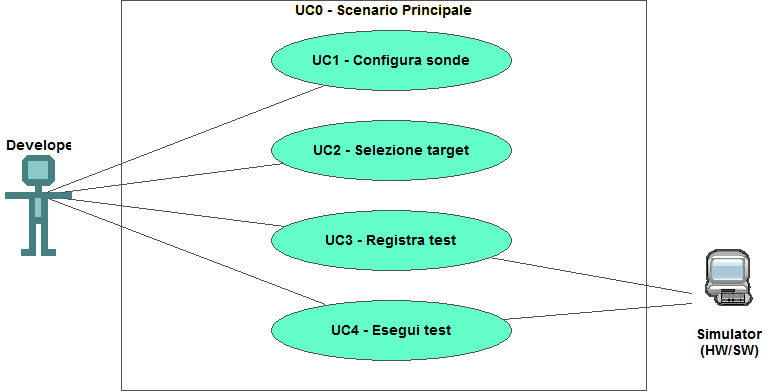
\includegraphics[width=0.9\columnwidth]{usecase/scenario-principale} 
%     \caption{Use Case - UC0: Scenario principale}
% \end{figure}

% \begin{usecase}{0}{Scenario principale}
% \usecaseactors{Sviluppatore applicativi}
% \usecasepre{Lo sviluppatore è entrato nel plug-in di simulazione all'interno dell'IDE}
% \usecasedesc{La finestra di simulazione mette a disposizione i comandi per configurare, registrare o eseguire un test}
% \usecasepost{Il sistema è pronto per permettere una nuova interazione}
% \label{uc:scenario-principale}
% \end{usecase}

% \section{Tracciamento dei requisiti}

% Da un'attenta analisi dei requisiti e degli use case effettuata sul progetto è stata stilata la tabella che traccia i requisiti in rapporto agli use case.\\
% Sono stati individuati diversi tipi di requisiti e si è quindi fatto utilizzo di un codice identificativo per distinguerli.\\
% Il codice dei requisiti è così strutturato R(F/Q/V)(N/D/O) dove:
% \begin{enumerate}
% 	\item[R =] requisito
%     \item[F =] funzionale
%     \item[Q =] qualitativo
%     \item[V =] di vincolo
%     \item[N =] obbligatorio (necessario)
%     \item[D =] desiderabile
%     \item[Z =] opzionale
% \end{enumerate}
% Nelle tabelle \ref{tab:requisiti-funzionali}, \ref{tab:requisiti-qualitativi} e \ref{tab:requisiti-vincolo} sono riassunti i requisiti e il loro tracciamento con gli use case delineati in fase di analisi.

% \newpage

% \begin{table}%
% \caption{Tabella del tracciamento dei requisti funzionali}
% \label{tab:requisiti-funzionali}
% \begin{tabularx}{\textwidth}{lXl}
% \hline\hline
% \textbf{Requisito} & \textbf{Descrizione} & \textbf{Use Case}\\
% \hline
% RFN-1     & L'interfaccia permette di configurare il tipo di sonde del test & UC1 \\
% \hline
% \end{tabularx}
% \end{table}%

% \begin{table}%
% \caption{Tabella del tracciamento dei requisiti qualitativi}
% \label{tab:requisiti-qualitativi}
% \begin{tabularx}{\textwidth}{lXl}
% \hline\hline
% \textbf{Requisito} & \textbf{Descrizione} & \textbf{Use Case}\\
% \hline
% RQD-1    & Le prestazioni del simulatore hardware deve garantire la giusta esecuzione dei test e non la generazione di falsi negativi & - \\
% \hline
% \end{tabularx}
% \end{table}%

% \begin{table}%
% \caption{Tabella del tracciamento dei requisiti di vincolo}
% \label{tab:requisiti-vincolo}
% \begin{tabularx}{\textwidth}{lXl}
% \hline\hline
% \textbf{Requisito} & \textbf{Descrizione} & \textbf{Use Case}\\
% \hline
% RVO-1    & La libreria per l'esecuzione dei test automatici deve essere riutilizzabile & - \\
% \hline
% \end{tabularx}
% \end{table}%
